% Chapter 5

\chapter{Evaluation and Results} % Main chapter title

\label{resu} % For referencing the chapter elsewhere, use \ref{Chapter1}

% \lhead{Chapter 6. \emph{Evaluation and Results}} % This is for the header on each page - perhaps a shortened title
The data collected from the study was processed and compiled to extract information aimed at evaluating the effectiveness of the integration of a casual game as part of the gamification strategy. The evaluation was done in terms of user engagement, which required the definition of some metrics. These metrics provided insights into the behaviour of users in every group. Then, a hypothesis testing showed that the user engagement did not present a statistically significant variation between the control and experimental groups.

%----------------------------------------------------------------------------------------
\section{User Engagement Metrics}
Evaluating the solution in terms of user engagement required the definition of some metrics. There are many alternatives to measure user engagement in mobile applications. The selection of one option over others depends on the aim of every application. As seen in Section \ref{desi-components-interest}, the core element of AnkiDroid is the flashcard reviewer. This component is where users get the benefits from the effects of spaced repetition. Therefore, the metrics of use for user engagement are defined around the actions and parameters that depended on the interactions done in this element.

Based on the original functionality of the flashcard reviewer, the first metric was the total number of flashcards reviewed during the period of study. This metric included the repetitions of flashcards since they are the foundations of the spaced repetition technique. Thus, the metric did not consider the performance of users. In other words, it did not penalise users based on their previous knowledge or ability to learn new things.

The flashcard reviewed was modified to include the earning of coins and points. These two parameters were also considered for the evaluation since they gave additional information about the number of flashcards. It is important to note that, as expressed in Equations \ref{eq:coins-formula} and \ref{eq:points-formula}, the number of points and coins depended on the time reviewing flashcards, which complemented the information from the total number of cards.

The total number of flashcards reviewed by each user depends on the amount of content of every flashcard. Since users were free to review flashcards based on their interests, chances are that they did not use the same decks. Therefore, the number of flashcards might not provide enough information. For this reason, another metric of use was the amount of time (measured in seconds) reviewing flashcards. This information was somehow encapsulated in the number of coins and points, but as seen in Equations \ref{eq:coins-formula} and \ref{eq:points-formula}, some flashcards could have given zero points and coins.

Other important metrics obtained from the compiled logs included the number of interactions, days using the application, average interactions per day (AIPD), the period of use, average time between sessions (ATBS), and the number of decks. The values of these metrics are detailed in Tables \ref{tab:summ_control} and \ref{tab:summ_experimental}. At a glance, the values are better for the experimental group, e.g., the number of reviewed flashcards is visually higher for the experimental group as seen in Figures \ref{fig:cards-control} and \ref{fig:cards-experimental}. However, these comparisons are not enough to evaluate the user engagement.

\begin{table*}[!htb]
    \centering
    \small
    \vspace{1cm}
    {\renewcommand{\arraystretch}{1}
        \begin{tabular}{|R{4.5cm}|R{1cm}|R{1cm}|R{1cm}|R{1cm}|R{1cm}|R{1cm}|}
        \hline
        \multicolumn{1}{|>{\arraybackslash}m{4.5cm}|}{\textbf{Participant}} &
        \multicolumn{1}{>{\centering\arraybackslash}m{1cm}|}{1} &
        \multicolumn{1}{>{\centering\arraybackslash}m{1cm}|}{2} &
        \multicolumn{1}{>{\centering\arraybackslash}m{1cm}|}{3} &
        \multicolumn{1}{>{\centering\arraybackslash}m{1cm}|}{4} &
        \multicolumn{1}{>{\centering\arraybackslash}m{1cm}|}{5} &
        \multicolumn{1}{>{\centering\arraybackslash}m{1cm}|}{6} \\
        \hline
        \textbf{Total cards} & 738 & 125 & 51 & 40 & 37 & 0 \\ \hline
        \textbf{Total points} & 1990 & 263 & 402 & 131 & 252 & 0 \\ \hline
        \textbf{Total coins} & 818 & 93 & 173 & 54 & 105 & 0 \\ \hline
        \textbf{Time in cards (seconds)} & 2317 & 386 & 354 & 143 & 223 & 0 \\ \hline
        \textbf{Interactions} & 1532 & 266 & 106 & 88 & 83 & 2 \\ \hline
        \textbf{Days using app} & 12 & 5 & 2 & 2 & 3 & 1 \\ \hline
        \textbf{Period of use (days)} & 22 & 11 & 8 & 2 & 8 & 1 \\ \hline
        \textbf{Decks} & 3 & 3 & 3 & 3 & 2 & 1 \\ \hline
        \textbf{AIPD} & 128 & 53 & 53 & 44 & 28 & 2 \\ \hline
        \textbf{ATBS (days)} & 1.8 & 2.2 & 4 & 1 & 2.6 & 1 \\ \hline
        \end{tabular}
    }
    \caption{User engagement metrics per user in control group.}
    \label{tab:summ_control}
\end{table*}

\begin{table*}[!htb]
    \centering
    \small
    \vspace{1cm}
    {\renewcommand{\arraystretch}{1}
        \begin{tabular}{|R{4.5cm}|R{1cm}|R{1cm}|R{1cm}|R{1cm}|R{1cm}|R{1cm}|}
        \hline
        \multicolumn{1}{|>{\arraybackslash}m{4.5cm}|}{\textbf{Participant}} &
        \multicolumn{1}{>{\centering\arraybackslash}m{1cm}|}{1} &
        \multicolumn{1}{>{\centering\arraybackslash}m{1cm}|}{2} &
        \multicolumn{1}{>{\centering\arraybackslash}m{1cm}|}{3} &
        \multicolumn{1}{>{\centering\arraybackslash}m{1cm}|}{4} &
        \multicolumn{1}{>{\centering\arraybackslash}m{1cm}|}{5} &
        \multicolumn{1}{>{\centering\arraybackslash}m{1cm}|}{6} \\
        \hline
        \textbf{Total cards} & 745 & 625 & 370 & 114 & 74 & 51\\ \hline
        \textbf{Total points} & 6221 & 1152 & 1311 & 1489 & 447 & 211\\ \hline
        \textbf{Total coins} & 2169 & 449 & 549 & 460 & 163 & 78\\ \hline
        \textbf{Time in cards (seconds)} & 7826 & 1495 & 1252 & 2433 & 554 & 252\\ \hline
        \textbf{Interactions} & 1699 & 1301 & 1250 & 294 & 180 & 114\\ \hline
        \textbf{Days using app} & 12 & 9 & 28 & 6 & 7 & 3\\ \hline
        \textbf{Period of use (days)} & 18 & 14 & 28 & 12 & 22 & 3\\ \hline
        \textbf{Decks} & 16 & 4 & 4 & 5 & 3 & 2\\ \hline
        \textbf{AIPD} & 142 & 145 & 45 & 49 & 26 & 38\\ \hline
        \textbf{ATBS (days)} & 1.5 & 1.5 & 1 & 2 & 3.1 & 1\\ \hline
        \end{tabular}
    }
    \caption{User engagement metrics per user in experimental group.}
    \label{tab:summ_experimental}
\end{table*}

\begin{figure}[htb]
    \vskip 5mm
        \begin{center}
            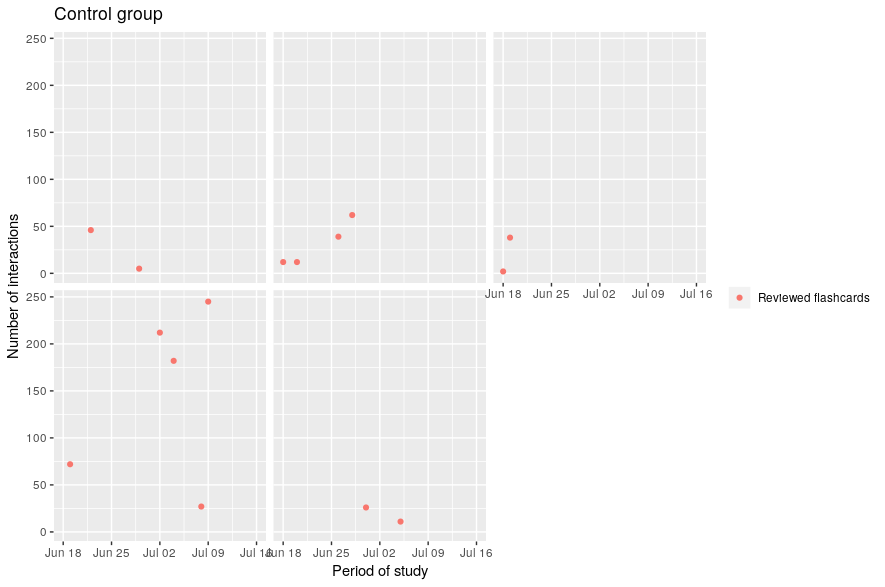
\includegraphics[scale=0.75]{./Figures/con_n_flashcards.png}
            \caption{Number of reviewed flashcards per user in the control group.}
            \label{fig:cards-control}
        \end{center}
    \vskip -5mm
\end{figure}

\begin{figure}[htb]
    \vskip 5mm
        \begin{center}
            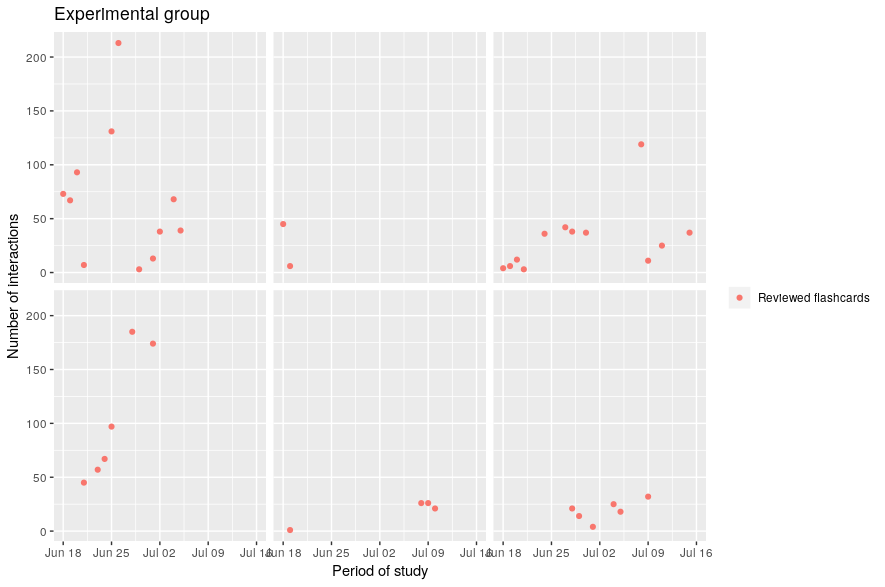
\includegraphics[scale=0.75]{./Figures/exp_n_flashcards.png}
            \caption{Number of reviewed flashcards per user in the experimental group.}
            \label{fig:cards-experimental}
        \end{center}
    \vskip -5mm
\end{figure}

%----------------------------------------------------------------------------------------
\section{Hypothesis Testing}
The proposed solution was designed to implement a gamification strategy that integrated a casual game. The objective was to provide users another extrinsic motivational element aimed at increasing user engagement. In other words, the goal of the project was the integration of a casual game as part of the gamification strategy to increase user engagement. Specifically, the hypothesis for the study was formulated as follows:

\begin{displayquote}
\textbf{User engagement is higher in the experimental group than in the control group.}
\end{displayquote}

The hypothesis was tested using the Student's t-test analysis over the defined user engagement metrics. This required defining the null hypothesis as follows:

\begin{displayquote}
\textbf{User engagement does not differ in the experimental group and the control groups.}
\end{displayquote}

The results of the t-test are shown in Table \ref{tab:t_test}. As can be seen, the majority of mean absolute values are larger in the experimental group. However, the p-values are not significantly small, which means that the null hypothesis could not be rejected. Moreover, the intervals of confidence at 95\% confirm that the results are not statistically significant, as seen in Figure \ref{fig:metrics}. Therefore, the difference of the means for every metric were due to chance. Thus, it was not possible to conclude that user engagement was affected by the integration of a casual game in a gamification strategy. Similar results were obtained from the data collected from users of a broader audience as seen in Table \ref{tab:t_test_broader}.


\begin{table*}[!htb]
    \centering
    \small
    \vspace{1cm}
    {\renewcommand{\arraystretch}{1}
        \begin{tabular}{|R{4.5cm}|R{1.5cm}|R{1.5cm}|R{1cm}|R{1cm}|}
        \hline
        \multicolumn{1}{|>{\arraybackslash}m{4.5cm}|}{\textbf{Metric}} &
        \multicolumn{1}{>{\centering\arraybackslash}m{2cm}|}{$\mu$ CG} &
        \multicolumn{1}{>{\centering\arraybackslash}m{2cm}|}{$\mu$ EG} &
        \multicolumn{1}{>{\centering\arraybackslash}m{2cm}|}{t-value} &
        \multicolumn{1}{>{\centering\arraybackslash}m{2cm}|}{p-value} \\
        \hline
        \textbf{Total cards} & 65.2 & 329.8 & -0.98 & 0.35\\ \hline
        \textbf{Total points} & 506.3 & 1805.2 & -1.36 & 0.22\\ \hline
        \textbf{Total coins} & 207.2 & 644.7 & -1.29 & 0.24\\ \hline
        \textbf{Time in cards (seconds)} & 570.5 & 2302 & -1.44 & 0.20\\ \hline
        \textbf{Interactions} & 346.2 & 806.3 & -1.25 & 0.24\\ \hline
        \textbf{Days using app} & 4.2 & 10.8 & -1.66 & 0.14\\ \hline
        \textbf{Period of use (days)} & 8.7 & 16.2 & -1.60 & 0.14\\ \hline
        \textbf{Decks} & 2.5 & 5.7 & -1.48 & 0.20\\ \hline
        \textbf{AIPD} & 51.3 & 74.2 & -0.81 & 0.43\\ \hline
        \textbf{ATBD (days)} & 2.1 & 1.7 & 0.74 & 0.48\\ \hline
        \end{tabular}
    }
    \caption{T-test values for user engagement metrics in the study groups. CG stands for control group, EG stands for experimental group.}
    \label{tab:t_test}
\end{table*}

\begin{table*}[!htb]
    \centering
    \small
    \vspace{1cm}
    {\renewcommand{\arraystretch}{1}
        \begin{tabular}{|R{4.5cm}|R{1.5cm}|R{1.5cm}|R{1cm}|R{1cm}|}
        \hline
        \multicolumn{1}{|>{\arraybackslash}m{4.5cm}|}{\textbf{Metric}} &
        \multicolumn{1}{>{\centering\arraybackslash}m{2cm}|}{$\mu$ AP} &
        \multicolumn{1}{>{\centering\arraybackslash}m{2cm}|}{$\mu$ AG} &
        \multicolumn{1}{>{\centering\arraybackslash}m{2cm}|}{t-value} &
        \multicolumn{1}{>{\centering\arraybackslash}m{2cm}|}{p-value} \\
        \hline
        \textbf{Total cards} & 1815.42 & 524.67 & 0.74 & 0.48\\ \hline
        \textbf{Total points} & 14156.33 & 5087.10 & 0.58 & 0.57\\ \hline
        \textbf{Total coins} & 5106.25 & 1676.92 & 0.68 & 0.50\\ \hline
        \textbf{Time in cards (seconds)} & 15493.33 & 10400.92 & 0.30 & 0.77\\ \hline
        \textbf{Interactions} & 3707 & 1126.5 & 0.72 & 0.49\\ \hline
        \textbf{Days using app} & 5.33 & 5.83 & -0.13 & 0.90\\ \hline
        \textbf{Period of use (days)} & 8.58 & 6.50 & 0.48 & 0.63\\ \hline
        \textbf{Decks} & 3.75 & 3.5 & 0.14 & 0.89\\ \hline
        \textbf{AIPD} & 178.5 & 50.25 & 0.91 & 0.38\\ \hline
        \textbf{ATBS (days)} & 1.90 & 1.08 & 1.83 & 0.09\\ \hline
        \end{tabular}
    }
    \caption{T-test values for user engagement metrics in the broader audience. AP stands for AnkiPlay, AG stands for AnkiGame.}
    \label{tab:t_test_broader}
\end{table*}

\begin{figure}[htb]
    \vskip 5mm
        \begin{center}
            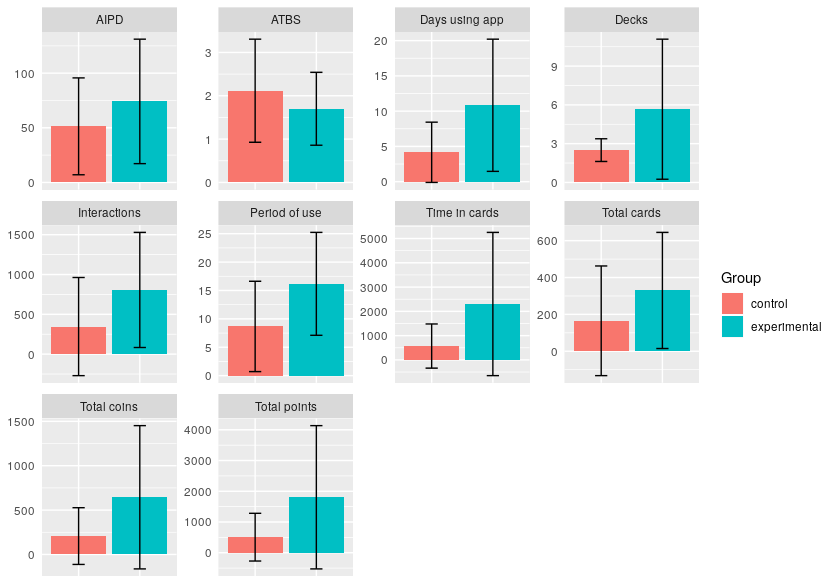
\includegraphics[scale=0.75]{./Figures/metrics.png}
            \caption{Means and intervals of confidence at 95\% for every metric.}
            \label{fig:metrics}
        \end{center}
    \vskip -5mm
\end{figure}